\documentclass[landscape]{article}
\usepackage[margin=0.5cm]{geometry}
\usepackage{pgfplots}
\pgfplotsset{compat=1.18}

\begin{document}

\begin{figure}
\centering
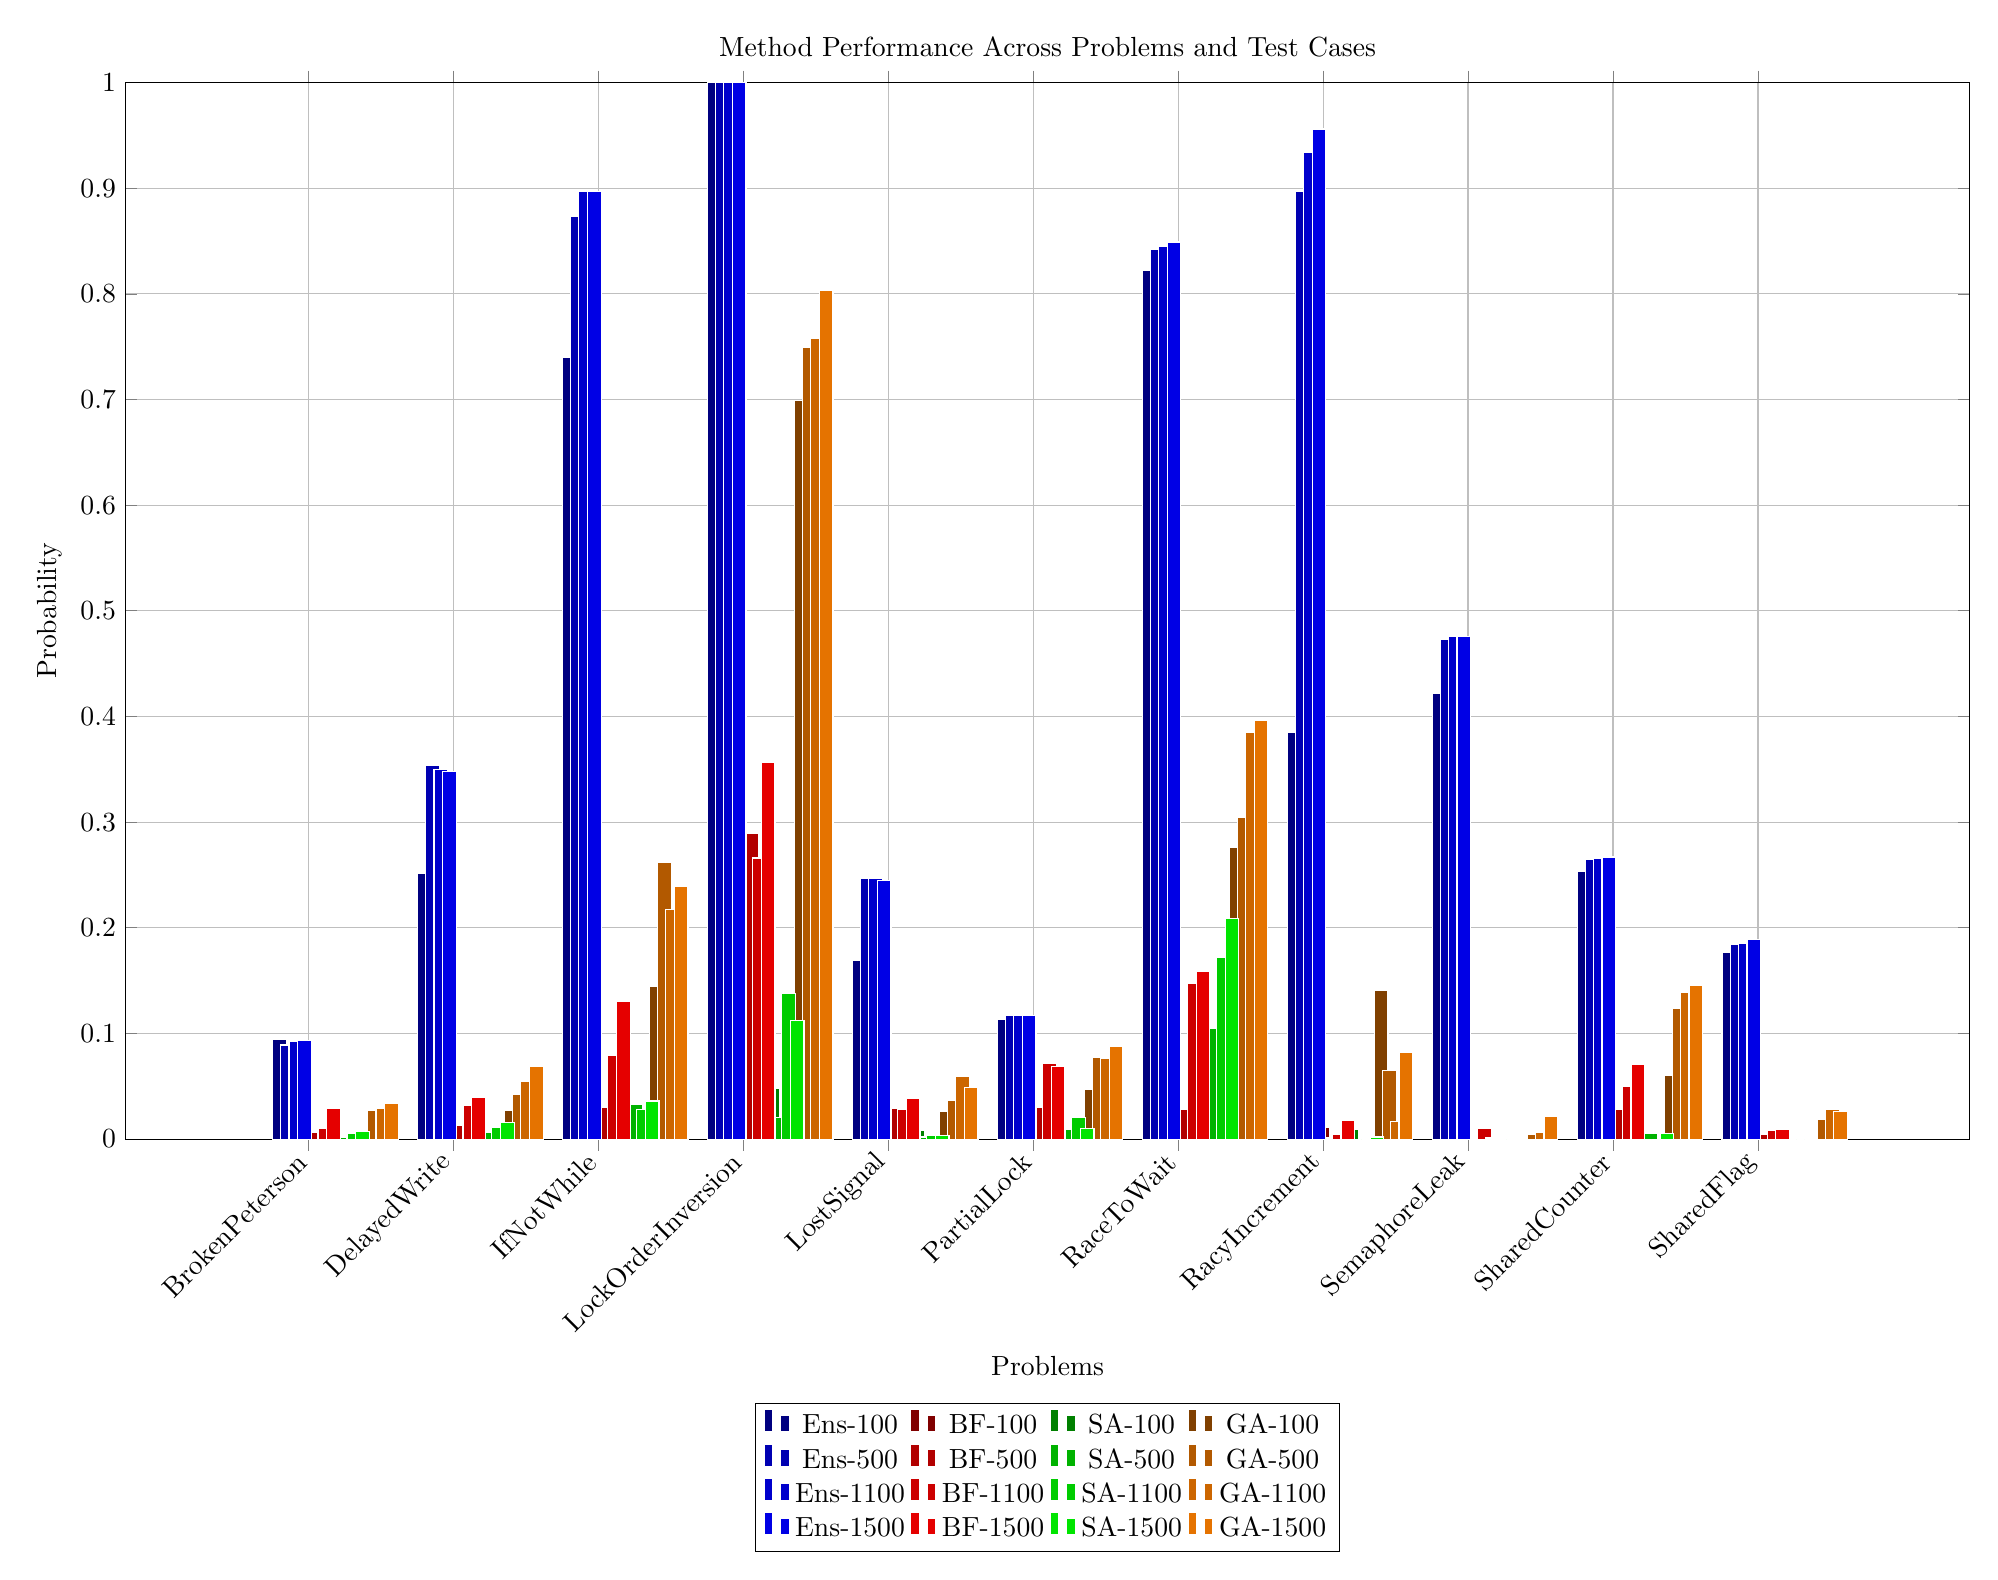
\begin{tikzpicture}
\begin{axis}[
    ybar,
    bar width=5pt,
    width=25cm,
    height=15cm,
    symbolic x coords={BrokenPeterson-Ens, BrokenPeterson-BF, BrokenPeterson-SA, BrokenPeterson-GA, spacer1, DelayedWrite-Ens, DelayedWrite-BF, DelayedWrite-SA, DelayedWrite-GA, spacer2, IfNotWhile-Ens, IfNotWhile-BF, IfNotWhile-SA, IfNotWhile-GA, spacer3, LockOrderInversion-Ens, LockOrderInversion-BF, LockOrderInversion-SA, LockOrderInversion-GA, spacer4, LostSignal-Ens, LostSignal-BF, LostSignal-SA, LostSignal-GA, spacer5, PartialLock-Ens, PartialLock-BF, PartialLock-SA, PartialLock-GA, spacer6, RaceToWait-Ens, RaceToWait-BF, RaceToWait-SA, RaceToWait-GA, spacer7, RacyIncrement-Ens, RacyIncrement-BF, RacyIncrement-SA, RacyIncrement-GA, spacer8, SemaphoreLeak-Ens, SemaphoreLeak-BF, SemaphoreLeak-SA, SemaphoreLeak-GA, spacer9, SharedCounter-Ens, SharedCounter-BF, SharedCounter-SA, SharedCounter-GA, spacer10, SharedFlag-Ens, SharedFlag-BF, SharedFlag-SA, SharedFlag-GA},
    xtick={BrokenPeterson-BF, DelayedWrite-BF, IfNotWhile-BF, LockOrderInversion-BF, LostSignal-BF, PartialLock-BF, RaceToWait-BF, RacyIncrement-BF, SemaphoreLeak-BF, SharedCounter-BF, SharedFlag-BF},
    xticklabels={BrokenPeterson, DelayedWrite, IfNotWhile, LockOrderInversion, LostSignal, PartialLock, RaceToWait, RacyIncrement, SemaphoreLeak, SharedCounter, SharedFlag},
    x tick label style={rotate=45, anchor=east},
    xlabel={Problems},
    ylabel={Probability},
    title={Method Performance Across Problems and Test Cases},
    legend style={at={(0.5,-0.25)}, anchor=north, legend columns=4},
    ymin=0,
    ymax=1,
    grid=major
]

\addplot+[
    bar shift=0pt,
    draw=white,
    fill=black!50!blue
] coordinates {
    (BrokenPeterson-Ens, 0.094) (DelayedWrite-Ens, 0.251) (IfNotWhile-Ens, 0.740) (LockOrderInversion-Ens, 1.000) (LostSignal-Ens, 0.169) (PartialLock-Ens, 0.113) (RaceToWait-Ens, 0.822) (RacyIncrement-Ens, 0.385) (SemaphoreLeak-Ens, 0.422) (SharedCounter-Ens, 0.253) (SharedFlag-Ens, 0.177)
};

\addplot+[
    bar shift=0pt,
    draw=white,
    fill=black!50!red
] coordinates {
    (BrokenPeterson-BF, 0.006) (DelayedWrite-BF, 0.009) (IfNotWhile-BF, 0.011) (LockOrderInversion-BF, 0.042) (LostSignal-BF, 0.010) (PartialLock-BF, 0.016) (RaceToWait-BF, 0.014) (RacyIncrement-BF, 0.011) (SemaphoreLeak-BF, 0.000) (SharedCounter-BF, 0.002) (SharedFlag-BF, 0.000)
};

\addplot+[
    bar shift=0pt,
    draw=white,
    fill=black!50!green
] coordinates {
    (BrokenPeterson-SA, 0.002) (DelayedWrite-SA, 0.003) (IfNotWhile-SA, 0.001) (LockOrderInversion-SA, 0.048) (LostSignal-SA, 0.008) (PartialLock-SA, 0.004) (RaceToWait-SA, 0.013) (RacyIncrement-SA, 0.009) (SemaphoreLeak-SA, 0.000) (SharedCounter-SA, 0.000) (SharedFlag-SA, 0.000)
};

\addplot+[
    bar shift=0pt,
    draw=white,
    fill=black!50!orange
] coordinates {
    (BrokenPeterson-GA, 0.005) (DelayedWrite-GA, 0.027) (IfNotWhile-GA, 0.144) (LockOrderInversion-GA, 0.699) (LostSignal-GA, 0.026) (PartialLock-GA, 0.047) (RaceToWait-GA, 0.276) (RacyIncrement-GA, 0.141) (SemaphoreLeak-GA, 0.000) (SharedCounter-GA, 0.060) (SharedFlag-GA, 0.001)
};

\addplot+[
    bar shift=3pt,
    draw=white,
    fill=black!30!blue
] coordinates {
    (BrokenPeterson-Ens, 0.089) (DelayedWrite-Ens, 0.354) (IfNotWhile-Ens, 0.873) (LockOrderInversion-Ens, 1.000) (LostSignal-Ens, 0.247) (PartialLock-Ens, 0.117) (RaceToWait-Ens, 0.842) (RacyIncrement-Ens, 0.897) (SemaphoreLeak-Ens, 0.473) (SharedCounter-Ens, 0.265) (SharedFlag-Ens, 0.184)
};

\addplot+[
    bar shift=3pt,
    draw=white,
    fill=black!30!red
] coordinates {
    (BrokenPeterson-BF, 0.006) (DelayedWrite-BF, 0.013) (IfNotWhile-BF, 0.030) (LockOrderInversion-BF, 0.289) (LostSignal-BF, 0.029) (PartialLock-BF, 0.030) (RaceToWait-BF, 0.028) (RacyIncrement-BF, 0.001) (SemaphoreLeak-BF, 0.000) (SharedCounter-BF, 0.028) (SharedFlag-BF, 0.004)
};

\addplot+[
    bar shift=3pt,
    draw=white,
    fill=black!30!green
] coordinates {
    (BrokenPeterson-SA, 0.002) (DelayedWrite-SA, 0.006) (IfNotWhile-SA, 0.033) (LockOrderInversion-SA, 0.020) (LostSignal-SA, 0.002) (PartialLock-SA, 0.009) (RaceToWait-SA, 0.105) (RacyIncrement-SA, 0.000) (SemaphoreLeak-SA, 0.000) (SharedCounter-SA, 0.005) (SharedFlag-SA, 0.000)
};

\addplot+[
    bar shift=3pt,
    draw=white,
    fill=black!30!orange
] coordinates {
    (BrokenPeterson-GA, 0.027) (DelayedWrite-GA, 0.042) (IfNotWhile-GA, 0.262) (LockOrderInversion-GA, 0.749) (LostSignal-GA, 0.037) (PartialLock-GA, 0.077) (RaceToWait-GA, 0.304) (RacyIncrement-GA, 0.065) (SemaphoreLeak-GA, 0.004) (SharedCounter-GA, 0.124) (SharedFlag-GA, 0.019)
};

\addplot+[
    bar shift=6pt,
    draw=white,
    fill=black!20!blue
] coordinates {
    (BrokenPeterson-Ens, 0.092) (DelayedWrite-Ens, 0.350) (IfNotWhile-Ens, 0.897) (LockOrderInversion-Ens, 1.000) (LostSignal-Ens, 0.247) (PartialLock-Ens, 0.117) (RaceToWait-Ens, 0.845) (RacyIncrement-Ens, 0.934) (SemaphoreLeak-Ens, 0.476) (SharedCounter-Ens, 0.266) (SharedFlag-Ens, 0.185)
};

\addplot+[
    bar shift=6pt,
    draw=white,
    fill=black!20!red
] coordinates {
    (BrokenPeterson-BF, 0.010) (DelayedWrite-BF, 0.032) (IfNotWhile-BF, 0.079) (LockOrderInversion-BF, 0.266) (LostSignal-BF, 0.028) (PartialLock-BF, 0.072) (RaceToWait-BF, 0.147) (RacyIncrement-BF, 0.004) (SemaphoreLeak-BF, 0.010) (SharedCounter-BF, 0.050) (SharedFlag-BF, 0.008)
};

\addplot+[
    bar shift=6pt,
    draw=white,
    fill=black!20!green
] coordinates {
    (BrokenPeterson-SA, 0.005) (DelayedWrite-SA, 0.011) (IfNotWhile-SA, 0.028) (LockOrderInversion-SA, 0.138) (LostSignal-SA, 0.003) (PartialLock-SA, 0.020) (RaceToWait-SA, 0.172) (RacyIncrement-SA, 0.000) (SemaphoreLeak-SA, 0.000) (SharedCounter-SA, 0.000) (SharedFlag-SA, 0.000)
};

\addplot+[
    bar shift=6pt,
    draw=white,
    fill=black!20!orange
] coordinates {
    (BrokenPeterson-GA, 0.029) (DelayedWrite-GA, 0.055) (IfNotWhile-GA, 0.217) (LockOrderInversion-GA, 0.758) (LostSignal-GA, 0.059) (PartialLock-GA, 0.076) (RaceToWait-GA, 0.385) (RacyIncrement-GA, 0.017) (SemaphoreLeak-GA, 0.006) (SharedCounter-GA, 0.139) (SharedFlag-GA, 0.028)
};

\addplot+[
    bar shift=9pt,
    draw=white,
    fill=black!10!blue
] coordinates {
    (BrokenPeterson-Ens, 0.093) (DelayedWrite-Ens, 0.348) (IfNotWhile-Ens, 0.897) (LockOrderInversion-Ens, 1.000) (LostSignal-Ens, 0.245) (PartialLock-Ens, 0.117) (RaceToWait-Ens, 0.849) (RacyIncrement-Ens, 0.956) (SemaphoreLeak-Ens, 0.476) (SharedCounter-Ens, 0.267) (SharedFlag-Ens, 0.189)
};

\addplot+[
    bar shift=9pt,
    draw=white,
    fill=black!10!red
] coordinates {
    (BrokenPeterson-BF, 0.029) (DelayedWrite-BF, 0.039) (IfNotWhile-BF, 0.130) (LockOrderInversion-BF, 0.356) (LostSignal-BF, 0.038) (PartialLock-BF, 0.069) (RaceToWait-BF, 0.159) (RacyIncrement-BF, 0.018) (SemaphoreLeak-BF, 0.001) (SharedCounter-BF, 0.071) (SharedFlag-BF, 0.009)
};

\addplot+[
    bar shift=9pt,
    draw=white,
    fill=black!10!green
] coordinates {
    (BrokenPeterson-SA, 0.007) (DelayedWrite-SA, 0.016) (IfNotWhile-SA, 0.036) (LockOrderInversion-SA, 0.112) (LostSignal-SA, 0.003) (PartialLock-SA, 0.010) (RaceToWait-SA, 0.209) (RacyIncrement-SA, 0.002) (SemaphoreLeak-SA, 0.000) (SharedCounter-SA, 0.005) (SharedFlag-SA, 0.000)
};

\addplot+[
    bar shift=9pt,
    draw=white,
    fill=black!10!orange
] coordinates {
    (BrokenPeterson-GA, 0.034) (DelayedWrite-GA, 0.069) (IfNotWhile-GA, 0.239) (LockOrderInversion-GA, 0.803) (LostSignal-GA, 0.049) (PartialLock-GA, 0.088) (RaceToWait-GA, 0.396) (RacyIncrement-GA, 0.082) (SemaphoreLeak-GA, 0.021) (SharedCounter-GA, 0.145) (SharedFlag-GA, 0.026)
};
\legend{Ens-100, BF-100, SA-100, GA-100, Ens-500, BF-500, SA-500, GA-500, Ens-1100, BF-1100, SA-1100, GA-1100, Ens-1500, BF-1500, SA-1500, GA-1500}

\end{axis}
\end{tikzpicture}
\caption{Method performance across problems with different test-case sizes.}
\end{figure}

\end{document}
